\documentclass[12pt]{article}
\usepackage{float}
\usepackage{graphicx}
\usepackage[fleqn]{amsmath}
\usepackage{amssymb}
\usepackage{parskip}
\usepackage[a4paper,top=2cm,bottom=2cm,left=3cm,right=3cm,marginparwidth=1.75cm]{geometry}

% \setlength{\parindent}{0pt}

\begin{document}

\date{}
\author{Marco Sterlini}

\title{Notes on Dynamic Triggering Mechanisms for Event-Triggered Control paper}

\maketitle

From \textbf{Dynamic Triggering Mechanisms for Event-Triggered Control} paper it is useful to extract the  dynamic ETM applied to the linear system case scenario:

$$
  \dot{x} = Ax + Bu, x \in \mathbb{R}^{n}, u \in \mathbb{R}^{m} 
$$

Assuming linear feedback controller $u = K x$ we obtain the ideal closed-loop system, we add the error considered in the paper e

$$
  \dot{x} = Ax + BK(x + e)
$$

That being asymptotically stable presents a Lyapunov function $V(x) = x^{\top} P x$ with $P$ p.d. and symmetric such That

$$
  (A + BK)^{\top}P + P(A + BK) = -Q
$$

We have then

\begin{multline*}
  \frac{d}{dt} V(x(t)) = \dot{x}^{\top} P x + x P \dot{x} = \\ 
  = (Ax + BKx + BKe)^{\top} P x + x^{\top} P (Ax + BKx + BKe) = \\
  = x^{\top} \left[ (A + BK)^{\top} P + P (A + BK) \right] x + x^{\top} P BKe + e^{\top} K^{\top} B^{\top} P x = \\
  \\
  \text{since the result is a scalar I can sum up the last two terms} \\
  \\
  = x^{\top} \left[ (A + BK)^{\top} P + P (A + BK) \right] x + 2 x^{\top} P B K e = - x^{\top} Q x + 2 x^{\top} P B K e
\end{multline*}

As a first approach the static ETM that follows can be used:

\begin{align} \label{static}
  t_0 &= 0, \nonumber \\
  t_{i+1} &= \text{inf} \left\{
  t \in \mathbb{R} | t > t_i \wedge \sigma x(t)^{\top} Q x(t) - 2 x(t)^{\top} P B K e(t^{-} ) \leq 0
  \right\}
\end{align}

This ensures that the next event will occur whenever the derivative of the Lyapunov function will cease to be negative. Ensuring a forced definite negativeness. 

\begin{figure}[H]
    \centering
    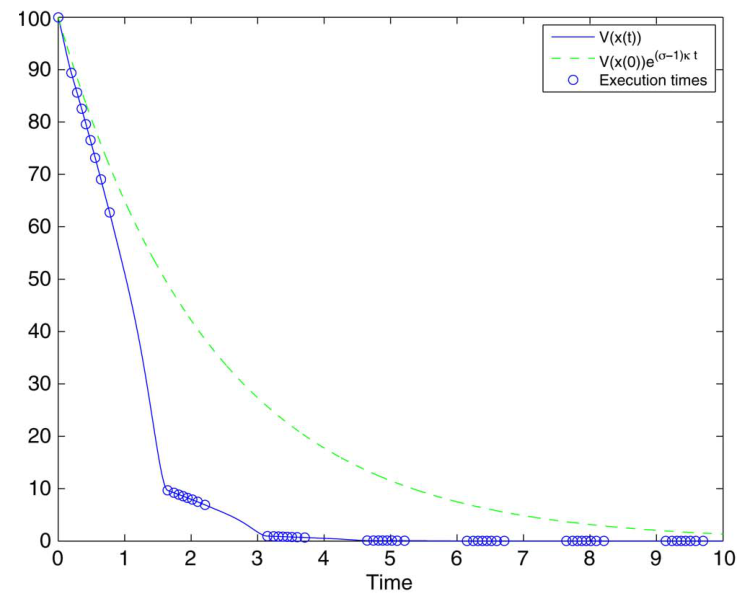
\includegraphics[width=0.65\textwidth]{img/static}
    \caption{It is clear how the Lyapunov function $V(x)$ is strictly decreasing}
    \label{static-plot}
\end{figure}


Now a dynamic ETM is proposed based on the dynamic variable $\eta$ governed by the differential equation

\begin{equation}
  \dot{\eta} = - \lambda \eta + \sigma x^{\top} Q x - 2 x^{\top} P B K e, \eta(0) = \eta_0
\end{equation}

With $\sigma \in \left( 0, 1 \right), \lambda > 0, \eta_0 \in \mathbb{R}^{+}_0$ the design parameters

It is important noticing how this addition of dynamic changes the overall behavior of the ETM mechanism. In the static case (equation. \ref{static}) the value is updated every time the condition is violated. By adding a dynamic term the update will not be immediate, $\eta(t)$ integrates the previous triggering signal over time rather than responding to the current value of the signal. The term $-\lambda \eta(t)$ makes $\eta(t)$ decay over time to that it doesn't accumulate the signal history indefinitely, it smoothly adjusts based on the previous value of the signal. Overall it's a filter of the previous signal since it gives a "smoothed" version of the signal used for the static ETM.

It is then defined the new dynamic ETM:


\begin{align} \label{dynamic}
  t_0 &= 0, \nonumber \\
  t_{i+1} &= \text{inf} \left\{
  t \in \mathbb{R} | t > t_i \wedge \eta(t) + \theta \left(  \sigma x(t)^{\top} Q x(t) - 2 x(t)^{\top} P B K e(t^{-} ) \right) \leq 0
  \right\}
\end{align}

It has been added the parameter $\theta \in \mathbb{R}^{+}_0$. The static ETM (equation. \ref{static}) can now be seen as the limit case scenario of the dynamic one (equation. \ref{dynamic}) where $\theta$ tends to $+ \infty$ and hence the $\eta(t)$ term can be ignored.

It is then proved how the inter-execution times with the dynamic ETM are larger with respect to the static ETM use. A new candidate Lyapunov function $W : \mathbb{R}^n \times \mathbb{R}_0^+ \to \mathbb{R}_0^+$ designed for the augmented system that sees the introduction of $e$ and $\eta$ variables:

\begin{equation}
  W(x, \eta) = V(x) + \eta 
\end{equation}

\begin{equation}
  \frac{d}{dt} W(x(t), \eta(t)) = \left( \sigma - 1 \right) x(t)^{\top} Q x(t) - \lambda \eta(t)
\end{equation}

That with the previous assumptions (not declared here but in the paper) that $\sigma \in \left( 0,1 \right)$ and $\eta(t) \geq 0$ with $\lambda > 0$ Assures that $\dot{W}$ stays definite negative and both $x(t)$ and $\eta(t)$ converge asymptotically to the origin.

It's then treated how each of the design parameters influence the overall system behavior. 3 different cases were portrayed where an explicit expression of the inter-execution time $\tau$ is drawn out.

It follows the treatment of the Lyapunov function decay rate, it is strongly influenced by $\sigma$, not influenced by $\theta$ and to understand the influence of this last term it has been used the \textit{Quadratic Integral Performance Index}.

To choose the parameters it was first tuned the Lyapunov function decay rate by imposing $\eta_0 = 0$ and $\lambda = (1 - \sigma) \kappa$ (what this $\kappa$ means it is explained in the paper), here $\sigma$ represents the degradation of Lyapunov function decay with respect to the ideal close-loop system. It was then chosen $\theta$ taking into account the considerations on $\tau$ formulation.

\textbf{Simulation results}

In comparison to the results of figure (fig. \ref{static-plot}) the dynamic ETM has been applied in the following:

\begin{figure}[H]
    \centering
    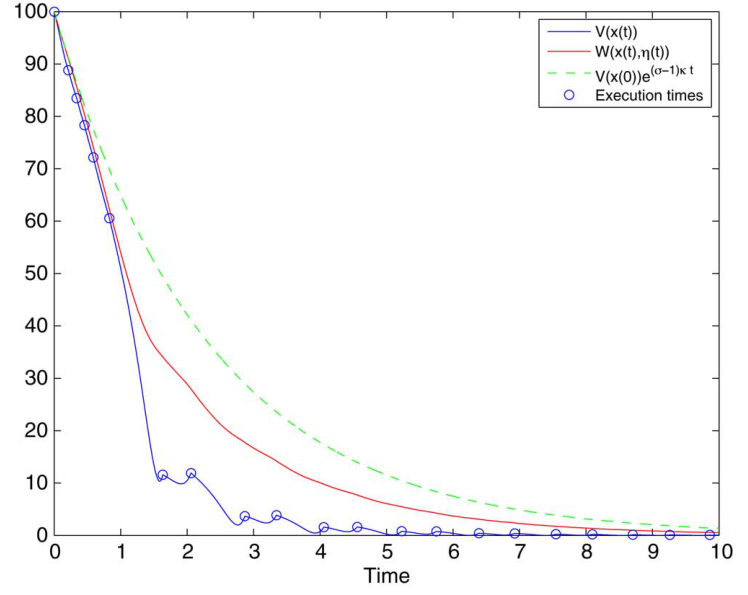
\includegraphics[width=0.65\textwidth]{img/dynamic}
    \caption{}
    \label{dynamic-plot}
\end{figure}

It was also done the comparison with a dynamic ETM taken from one of the references that worked as follows:

\begin{align}
  t_0 &= 0 \nonumber \\
  t_{i+1} &= \text{inf} \left\{ t \in \mathbb{R} | t > t_i \wedge V(x(t)) \geq e^{\left( \sigma - 1 \right) \kappa \left( t - t_i \right)} V(x(t_i)) \right\}
\end{align}

In this case the update will occur every time the value of the Lyapunov function will exceed the one of the exponential as shown in the following:

\begin{figure}[H]
    \centering
    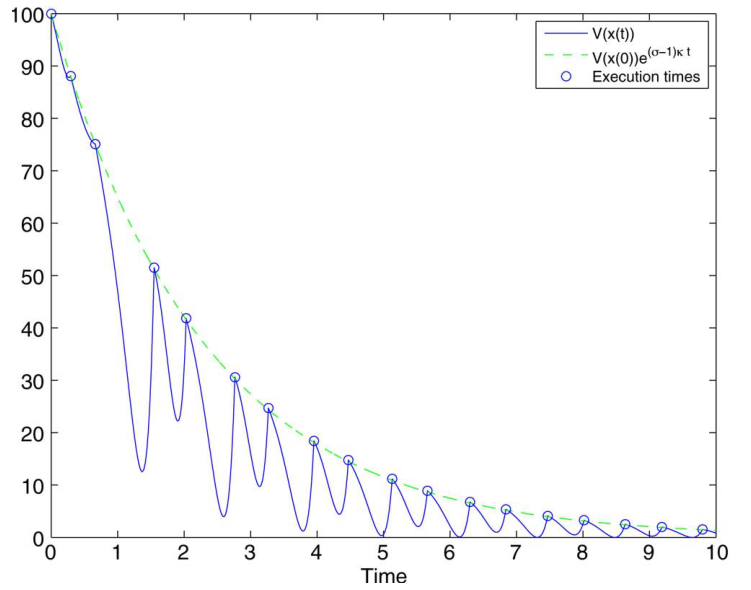
\includegraphics[width=0.65\textwidth]{img/reference}
    \caption{}
    \label{reference-plot}
\end{figure}

In the final comment it's shown how the approach of this paper puts itself as a good compromise between the good monotonic behavior of the static ETM and the large inter-execution times of the reference approach (fig. \ref{reference-plot}) that, however, exhibit large variations in $V$ value.

Also, it is shown that using a dynamic ETM the coefficient of variability of the inter-execution times is reduced by a lot, meaning that the controller acts in a more predictable way.

\end{document}

% \begin{figure}[H]
%     \centering
%     \begin{subfigure}{0.4\textwidth}
%     \includegraphics[width=\textwidth]{}
%     \caption{}
%     \label{}
%     \end{subfigure}
%     \hfill
%     \begin{subfigure}{0.55\textwidth}
%     \includegraphics[width=\textwidth]{}
%     \caption{}
%     \label{}
%     \end{subfigure}
%     \caption{}
%     \label{}
% \end{figure}

% \begin{figure}[H]
%     \centering
%     \includegraphics[width=0.65\textwidth]{}
%     \caption{}
%     \label{}
% \end{figure}